\documentclass[11pt]{article}

\usepackage[a4paper,margin=2.2cm]{geometry}
\usepackage{amsmath,amssymb}
\usepackage{graphicx}
\usepackage{subcaption}
\usepackage{booktabs}
\usepackage{siunitx}
\usepackage{xcolor}
\usepackage[hidelinks]{hyperref}
\usepackage{caption}
\captionsetup{font=small}

\newcommand{\ESC}{E_{S,C}}
\newcommand{\EI}{E_{I}}
\newcommand{\VBV}{V_{B,V}}
\newcommand{\epsI}{\varepsilon_{I}}
\newcommand{\epsS}{\varepsilon_{S}}
\newcommand{\sigin}{\sigma_{\mathrm{in}}}
\newcommand{\tS}{t_{S}}
\newcommand{\tI}{t_{I}}

\title{\vspace{-1.2cm}\textbf{Reproduction of Zhang, Li, Hu \& Luo (IEEE T-ED 2009)}\\[4pt]
\large ``Field Enhancement for Dielectric Layer of High-Voltage Devices on
Silicon on Insulator''\\ \normalsize IEEE Trans.\ Electron Devices \textbf{56}(10),
pp.~2327--2334 --- the ENDIF principle}
\author{Independent derivation, simulation and figure-by-figure comparison}
\date{}

\begin{document}
\maketitle
\vspace{-0.8cm}

\begin{abstract}
\noindent In an SOI high-voltage device the vertical breakdown is limited by the
\emph{silicon} critical field $\ESC$, but the buried \emph{dielectric} can sustain
a much larger field $\EI$ fixed by displacement continuity across the
silicon/dielectric interface. The ENDIF (enhanced dielectric-layer field)
principle raises $\EI$ --- and hence the vertical breakdown voltage $\VBV$ ---
through three knobs: (1)~a thin silicon layer (higher $\ESC$), (2)~a low-$k$
buried dielectric, and (3)~an interface sheet charge $\sigin$. This note derives
the closed-form model and reproduces the paper's analytical figures (Figs.~2--5).
All headline numbers match to within rounding.
\end{abstract}

\section*{Key results (model vs.\ paper)}
\begin{center}
\begin{tabular}{@{}lcc@{}}
\toprule
Quantity & Model & Paper \\
\midrule
$\ESC$ at $\tS=\SI{0.1}{\micro\meter}$ & \SI{140.8}{\volt\per\micro\meter} & \SI{141}{\volt\per\micro\meter} \\
$\EI$ at $\tS=\SI{1}{\micro\meter}$, $\epsI=3.9\varepsilon_0$, $\sigin=0$ & \SI{161}{\volt\per\micro\meter} & \SI{161}{\volt\per\micro\meter} \\
$\EI$ at $\tS=\SI{1}{\micro\meter}$, $\epsI=2.0\varepsilon_0$ (low-$k$) & \SI{313}{\volt\per\micro\meter} & \SI{319}{\volt\per\micro\meter} \\
$\EI$ at $\tS=\SI{0.1}{\micro\meter}$ & \SI{422}{\volt\per\micro\meter} & \SI{423}{\volt\per\micro\meter} \\
$\VBV$ at $\tS=\SI{1}{\micro\meter}$ & \SI{348}{\volt} & \SI{348}{\volt} \\
$\VBV$ at $\tS=\SI{0.1}{\micro\meter}$ & \SI{852}{\volt} & \SI{852}{\volt} \\
$\VBV$ at $\tS=\SI{1}{\micro\meter}$, $\sigin=\SI{4e12}{\per\square\centi\meter}$ & \SI{719}{\volt} & \SI{719}{\volt} \\
\bottomrule
\end{tabular}
\end{center}

\section{Theory}

\subsection{Displacement continuity: why the dielectric field is enhanced}
At the silicon/dielectric interface the normal electric displacement is continuous
up to any interface sheet charge $\sigin$:
\begin{equation}
\epsI \EI = \epsS \ESC + q\sigin
\;\;\Longrightarrow\;\;
\boxed{\;\EI = \frac{\epsS}{\epsI}\,\ESC + \frac{q\sigin}{\epsI}\;}
\end{equation}
Because $\epsS/\epsI \approx 11.7/3.9 \approx 3$, the dielectric already carries
$\sim\!3\times$ the silicon field; lowering $\epsI$ (low-$k$) or adding $\sigin$
raises it further. This is the ENDIF idea: the blocking capability is set by how
much field the \emph{buried dielectric} can hold, not the silicon.

\subsection{Silicon critical field vs.\ thickness}
Breakdown in the (thin, fully depleted) silicon occurs when the ionization
integral reaches unity. Carrying out that condition with the silicon Chynoweth
coefficient and the thin-layer field profile yields the paper's compact fit
(eq.~10), with $\tS$ in micrometres:
\begin{equation}
\ESC(\tS) = 9.783\,\frac{21.765 - \ln \tS}{\ln \tS + 3.975}\times 10^{4}
\ \ [\si{\volt\per\centi\meter}],
\end{equation}
which rises sharply for thin silicon --- reaching \SI{141}{\volt\per\micro\meter}
at $\tS=\SI{0.1}{\micro\meter}$, far above the conventional constant
\SI{20}{\volt\per\micro\meter}. The associated silicon critical ionization rate is
the Chynoweth rate evaluated at $\ESC$,
$\alpha_{S,C} = A\,e^{-B/\ESC}$ with $A=\SI{7.03e5}{\per\centi\meter}$,
$B=\SI{1.231e6}{\volt\per\centi\meter}$ (Fig.~2).

\subsection{Dielectric field and vertical breakdown voltage}
Substituting $\ESC(\tS)$ into the continuity relation gives $\EI(\tS,\epsI,\sigin)$
(eq.~11). Integrating the field through the silicon ($\tfrac12\epsI\tS$ effective)
and the dielectric ($\epsS\tI$) gives the vertical breakdown voltage (eq.~13), with
$\tS,\tI$ in micrometres and $\epsS,\epsI$ relative:
\begin{equation}
\VBV = \left\{
\left[\,9.783\,\frac{21.765-\ln\tS}{\ln\tS+3.975}\right]
\big(\epsS\tI + \tfrac12\epsI\tS\big)
+ q\sigin\tI\times10^{-4}
\right\}\Big/\epsI .
\end{equation}
$\VBV(\tS)$ is U-shaped: it rises for thin silicon (high $\ESC$) and again for thick
silicon (more voltage held in the silicon), with an optimum in between. Larger
$\sigin$ and smaller $\epsI$ shift the whole family upward.

\subsection{Enhancement factors}
Relative to a conventional device ($\ESC=\SI{20}{\volt\per\micro\meter}$,
$E_{I,\mathrm{Con}}=\SI{60}{\volt\per\micro\meter}$), the three knobs contribute
additively, $\Delta\gamma=\Delta\gamma_1+\Delta\gamma_2+\Delta\gamma_3$ (eq.~12):
\begin{equation}
\Delta\gamma_1 = \frac{\epsS\,\Delta\ESC}{\varepsilon_{SiO_2}E_{I,\mathrm{Con}}},
\quad
\Delta\gamma_2 = \frac{\Delta\epsI}{\varepsilon_{SiO_2}-\Delta\epsI},
\quad
\Delta\gamma_3 = \frac{q\sigin}{\varepsilon_{SiO_2}E_{I,\mathrm{Con}}} .
\end{equation}
Each reaches the target $\Delta\gamma_i=15.67$ (i.e.\ $\EI=\SI{1000}{\volt\per\micro\meter}$)
at $\tS\lesssim\SI{50}{\nano\meter}$, $\epsI=0.25\varepsilon_0$, or
$\sigin=\SI{2e13}{\per\square\centi\meter}$, respectively --- so satisfying
\emph{any one} condition suffices. Interface charge is the most practical knob.

\paragraph{Parameters.} $\epsS=11.7$, $\varepsilon_{SiO_2}=3.9$;
$A=\SI{7.03e5}{\per\centi\meter}$, $B=\SI{1.231e6}{\volt\per\centi\meter}$;
$\tI=\SI{2}{\micro\meter}$ (Figs.~3--5).

\section{Figure-by-figure comparison}

\begin{figure}[h!]
\centering
\begin{subfigure}{0.46\textwidth}
\includegraphics[width=\linewidth]{../figs_paper/fig2_paper.png}
\caption{Paper (original)}
\end{subfigure}\hfill
\begin{subfigure}{0.52\textwidth}
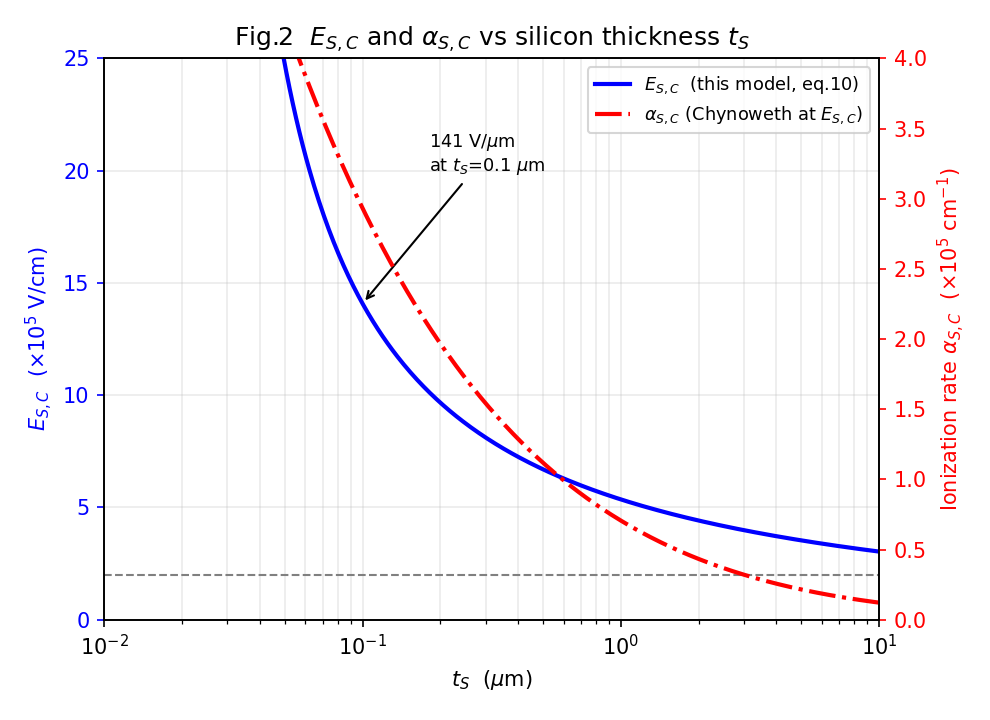
\includegraphics[width=\linewidth]{../figs/fig2_esc_alpha.png}
\caption{This reproduction}
\end{subfigure}
\caption{\textbf{Fig.~2 --- $\ESC$ and $\alpha_{S,C}$ vs.\ $\tS$.} The critical field
rises steeply for thin silicon (\SI{141}{\volt\per\micro\meter} at
\SI{0.1}{\micro\meter}); the critical ionization rate $\alpha_{S,C}$ (right axis,
Chynoweth at $\ESC$) grows as $\tS$ shrinks.}
\end{figure}

\begin{figure}[h!]
\centering
\begin{subfigure}{0.46\textwidth}
\includegraphics[width=\linewidth]{../figs_paper/fig3a_paper.png}
\caption{Paper (original)}
\end{subfigure}\hfill
\begin{subfigure}{0.52\textwidth}
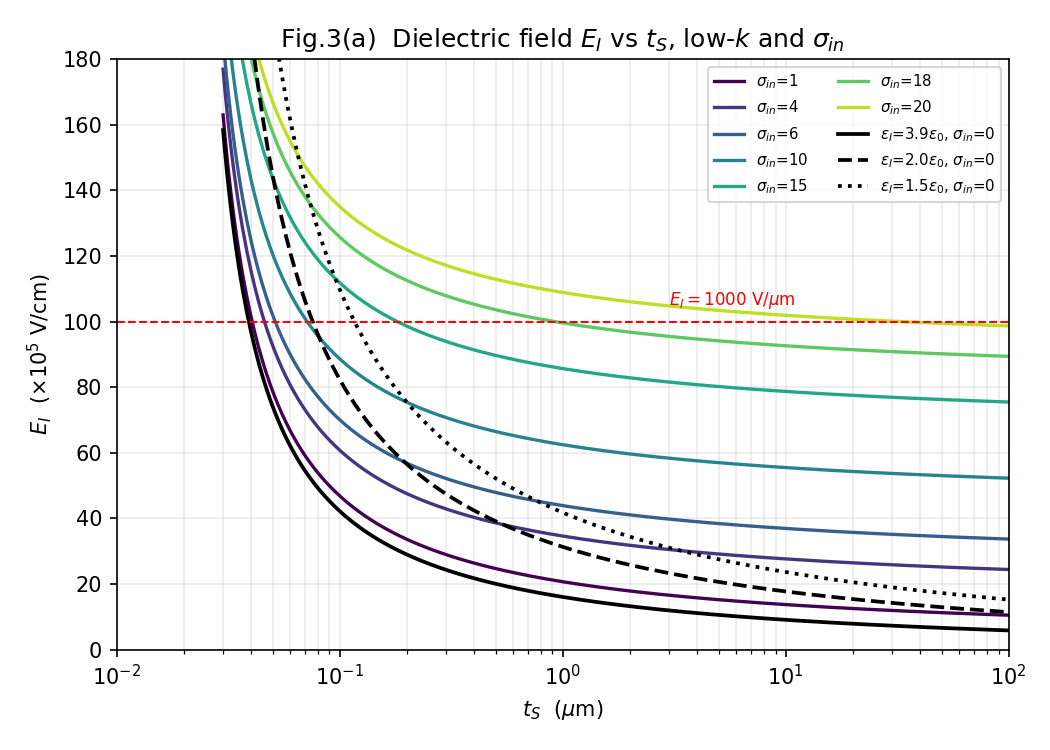
\includegraphics[width=\linewidth]{../figs/fig3a_EI.png}
\caption{This reproduction}
\end{subfigure}
\caption{\textbf{Fig.~3(a) --- dielectric field $\EI$ vs.\ $\tS$, low-$k$ and
$\sigin$.} Upper family: $\sigin=1$--$20\times10^{12}\,\si{\per\square\centi\meter}$
($\epsI=3.9\varepsilon_0$); lower black curves: $\epsI=3.9/2.0/1.5\,\varepsilon_0$
($\sigin=0$). Both knobs push $\EI$ toward the \SI{1000}{\volt\per\micro\meter}
dashed line.}
\end{figure}

\begin{figure}[h!]
\centering
\begin{subfigure}{0.46\textwidth}
\includegraphics[width=\linewidth]{../figs_paper/fig3b_paper.png}
\caption{Paper (original)}
\end{subfigure}\hfill
\begin{subfigure}{0.52\textwidth}
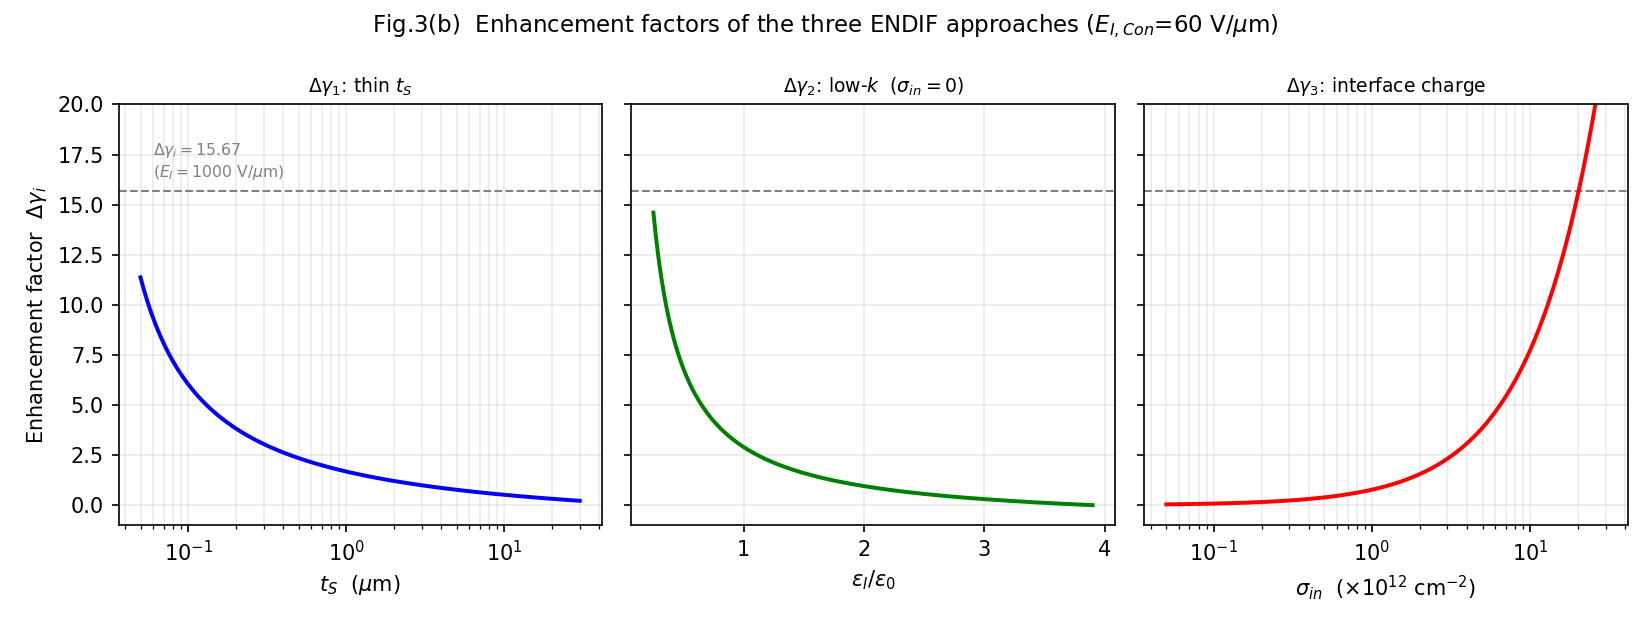
\includegraphics[width=\linewidth]{../figs/fig3b_enhancement.png}
\caption{This reproduction}
\end{subfigure}
\caption{\textbf{Fig.~3(b) --- enhancement factors $\Delta\gamma_i$.} Each approach
reaches $\Delta\gamma_i=15.67$ ($\EI=\SI{1000}{\volt\per\micro\meter}$) on its own:
thin $\tS$, low $\epsI$, or interface charge $\sigin$ (crossing at
$\sim\!\SI{2e13}{\per\square\centi\meter}$, matching the paper).}
\end{figure}

\begin{figure}[h!]
\centering
\begin{subfigure}{0.46\textwidth}
\includegraphics[width=\linewidth]{../figs_paper/fig4_paper.png}
\caption{Paper (original)}
\end{subfigure}\hfill
\begin{subfigure}{0.52\textwidth}
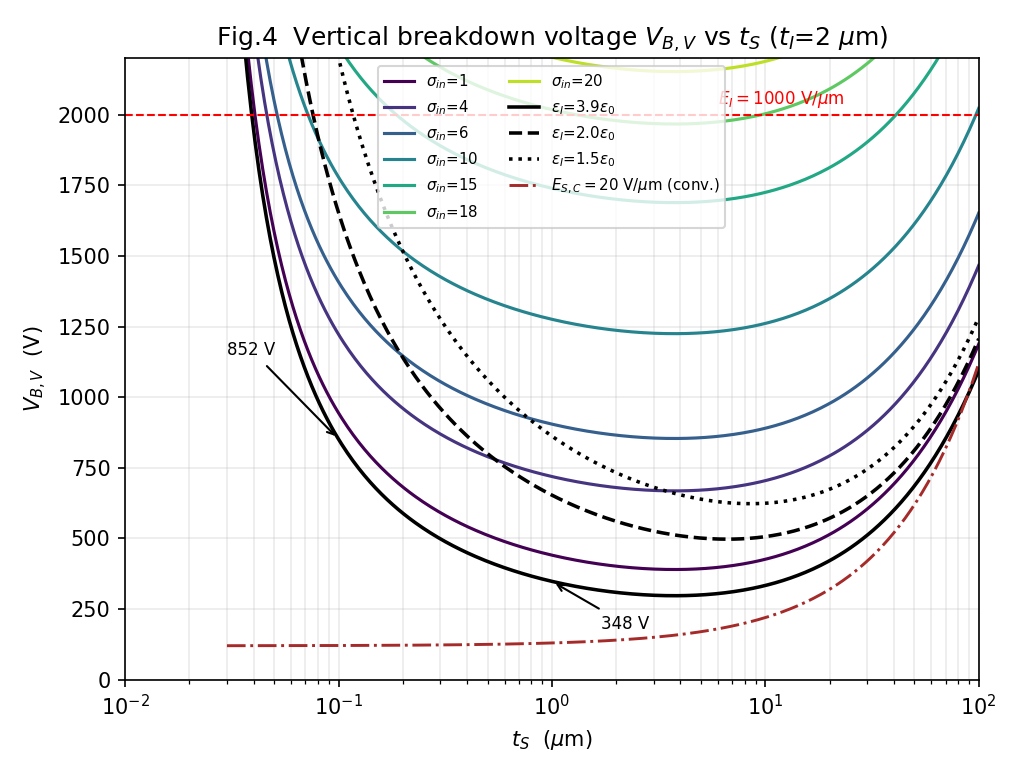
\includegraphics[width=\linewidth]{../figs/fig4_vbv.png}
\caption{This reproduction}
\end{subfigure}
\caption{\textbf{Fig.~4 --- vertical breakdown voltage $\VBV$ vs.\ $\tS$}
($\tI=\SI{2}{\micro\meter}$). U-shaped family; higher $\sigin$ / lower $\epsI$ lift
$\VBV$. The conventional $\ESC=\SI{20}{\volt\per\micro\meter}$ curve (bottom) is far
lower for thin silicon. Model $\VBV=348/852\,\si{\volt}$ at
$\tS=1/0.1\,\si{\micro\meter}$ match the paper exactly.}
\end{figure}

\begin{figure}[h!]
\centering
\begin{subfigure}{0.46\textwidth}
\includegraphics[width=\linewidth]{../figs_paper/fig5_paper.png}
\caption{Paper (original)}
\end{subfigure}\hfill
\begin{subfigure}{0.52\textwidth}
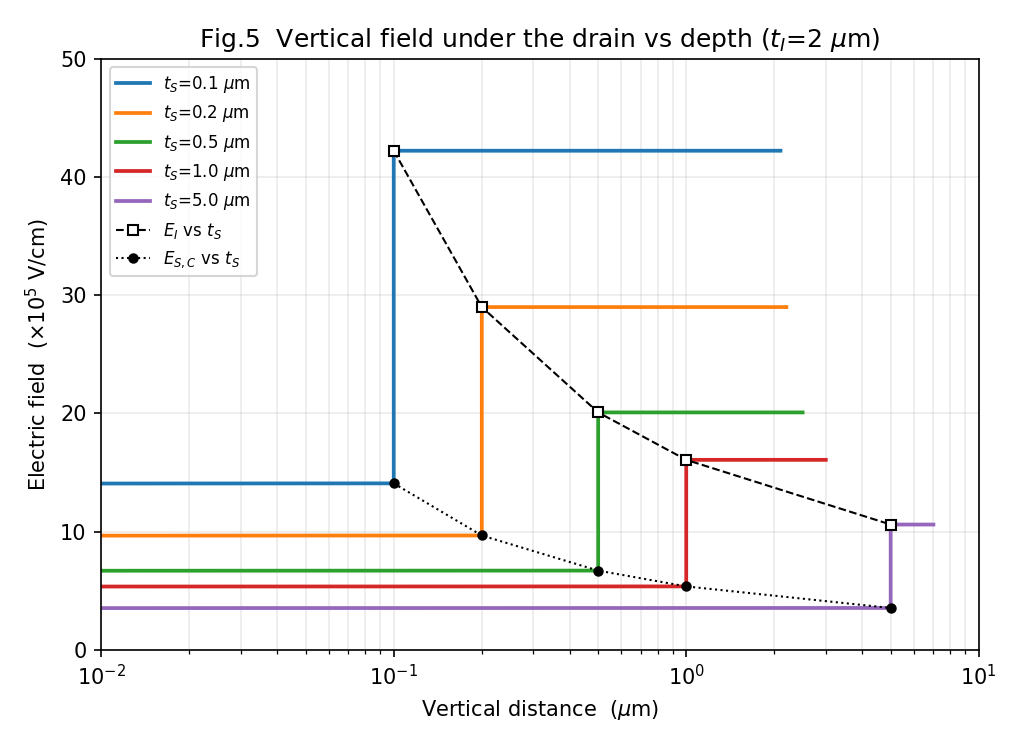
\includegraphics[width=\linewidth]{../figs/fig5_vertical_field.png}
\caption{This reproduction}
\end{subfigure}
\caption{\textbf{Fig.~5 --- vertical field under the drain vs.\ depth} for several
$\tS$. Each profile shows the silicon field limited to $\ESC$ then jumping to the
plateau $\EI$ across the buried dielectric; the two envelopes ($\EI$ and $\ESC$
vs.\ $\tS$) rise sharply for thin silicon.}
\end{figure}

\clearpage
\section{Notes and limitations}
\textbf{What matches:} the closed-form ENDIF quantities --- $\ESC(\tS)$,
$\alpha_{S,C}$, $\EI$, $\VBV$, and the enhancement factors --- reproduce the paper's
Figs.~2--5 and every stated number to within rounding.\\[4pt]
\textbf{Scope:} this reproduction covers the paper's \emph{analytical} core. Figs.~6--8
(step-thickness drift region, VK/LK SOI, and trench-SOI devices) are specific 2-D
device structures compared against MEDICI simulations and experiment; reproducing
those quantitatively requires a full 2-D device simulator and is out of scope here.\\[4pt]
\textbf{Erratum found in the paper's text:} the sentence ``when $\tS=\SI{1}{\micro\meter}$
and $\epsI=3.9\varepsilon_0$, $\EI$ values are 161 and \SI{681}{\volt\per\micro\meter} for
$\sigin$ of 0 and $4\times10^{12}\,\si{\per\square\centi\meter}$'' is internally
inconsistent: eq.~(11) gives $\EI = 161+186 = \SI{347}{\volt\per\micro\meter}$; the
paper's own $\VBV=\SI{719}{\volt}$ implies the same 347; and the paper's own
Fig.~3(a) $\sigin{=}4$ curve reads ${\sim}35\times10^{5}\,\si{\volt\per\centi\meter}$
at $\tS=\SI{1}{\micro\meter}$. The origin of 681 is identifiable: computing with the
\emph{low-$k$} permittivity $\epsI=2.0\varepsilon_0$ gives
$319+362=\SI{681}{\volt\per\micro\meter}$ exactly --- the LK value from the preceding
sentence was carried into the interface-charge example. Text-level typo only; all
equations and figures are mutually consistent (see \texttt{verify\_681.py}).\\[4pt]
\textbf{Code:} \texttt{zhang2009\_full.py} --- single file, closed-form model
$\to$ Figs.~2--5, with a self-check that prints all the headline numbers above;
\texttt{verify\_681.py} --- the three-way erratum verification.

\end{document}
